\documentclass[tikz,multi,border=10pt]{standalone}
\usetikzlibrary{shadows,arrows.meta,positioning,backgrounds,fit,chains,scopes}

% Define block styles
\tikzset{%
  materia/.style={draw, fill=cyan!20, text width=6.0em, text centered, minimum height=1.5em,drop shadow},
  etape/.style={materia, text width=8em, minimum width=10em, minimum height=3em, rounded corners, drop shadow},
  linepart/.style={draw, thick, color=black!50, -LaTeX, dashed},
  line/.style={draw, thick, color=black!50, -LaTeX},
  ur/.style={color=black, text centered, minimum height=0.01em},
  back group/.style={fill=yellow!20,rounded corners, draw=black!50, dashed, inner xsep=15pt, inner ysep=10pt},
}

\newcommand{\transreceptor}[3]{%
  \path [linepart] (#1.east) -- node [above] {\scriptsize #2} (#3);}

\begin{document}
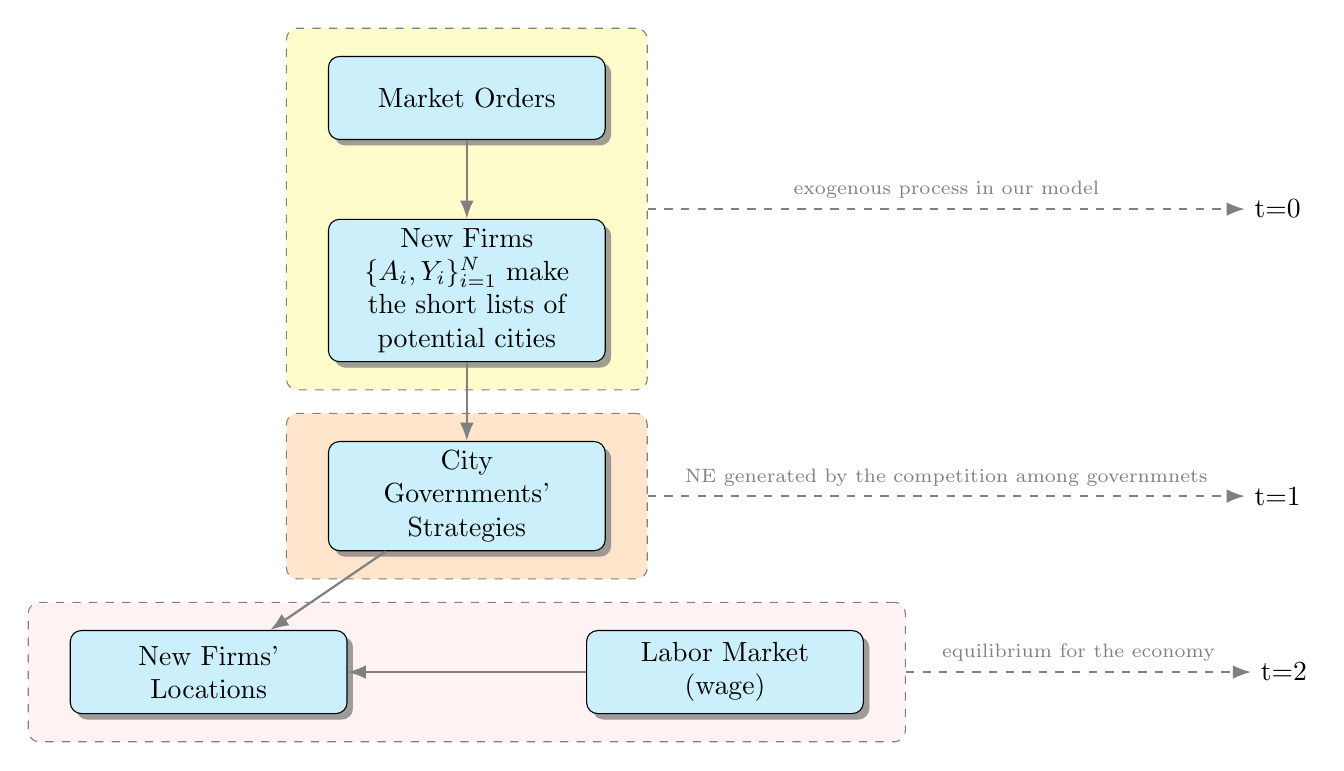
\begin{tikzpicture}
  [
  start chain=p going below,
  every on chain/.append style={etape},
  every join/.append style={line},
  node distance=1 and -.25,
  ]
  {
  \node [on chain, join] {Market Orders};
  \node [on chain, join] {New Firms $\{A_i, Y_i\}_{i=1}^{N}$ make the short lists of potential cities};
  \node [on chain, join] {City\\ Governments' Strategies};
  {[start branch=l going below left]
  \node [on chain] {New Firms' Locations};
  }
  {[start branch=r going below right]
  \node [on chain] {Labor Market\\ (wage)};
  }
  }

  \begin{scope}[on background layer]
    \node (bk1) [back group,fill=yellow!20] [fit=(p-1) (p-2)] {};
    \node (bk2) [back group,fill=orange!20] [fit=(p-3)] {};
    \node (bk3) [back group,fill=pink!20] [fit=(p/l-2) (p/r-2)] {};
  \end{scope}

  \path [line] (p-3) --  (p/l-2);
  %\path [line] (p-3) --  (p/r-2);
  \path [line] (p/r-2) --  (p/l-2);
  \path (bk1.east)+(+8.0,0) node (ur1)[ur] {t=0};
  \path (bk2.east)+(+8.0,0) node (ur2)[ur] {t=1};
  \path (bk3.east)+(+4.8,0) node (ur3)[ur] {t=2};


  \transreceptor{bk1}{exogenous process in our model}{ur1};
  \transreceptor{bk2}{NE generated by the competition among governmnets}{ur2};
  \transreceptor{bk3}{equilibrium for the economy}{ur3};
\end{tikzpicture}
\end{document}